\documentclass[11pt, a4paper]{article}

\usepackage[a4paper, width = 150 mm, top = 25 mm, bottom = 25 mm]{geometry}
\usepackage{amsfonts}
\usepackage{titlesec}
\usepackage{color}
\usepackage{graphicx}
\usepackage{subcaption}
\usepackage{float}
\usepackage{verbatim}
\usepackage[style=apa,backend=biber, citestyle=authoryear, sorting=nyt]{biblatex}
\addbibresource{references.bib}


\title{Controlling Player Avatars in Game Worlds using Multi-Modal Input Systems}
\author{Charlie Lloyd-Buckingham}
\date{\today}


\newcommand{\addfigure}[1]
{
\hfill 

\textcolor{red}{[Add Figure: #1]}

\hfill
}

\newcommand{\commentintext}[1]
{\hfill 

\textcolor{red}{#1} 
	
\hfill
}


\newcommand{\addcitation}{\textcolor{red}{[Citation Need]}}
\newcommand{\ccite}[1]{(\citeauthor{#1}, \citeyear{#1})}
\newcommand{\cciteyear}[1]{(\citeyear{#1})}
\newcommand{\cciteauthor}[1]{(\citeauthor{#1})}
\newcommand{\reffigure}[1]{Figure \ref{#1}}
\newcommand{\reftable}[1]{Table \ref{#1}}
\newcommand{\refequation}[1]{Equation \ref{#1}}

\begin{document}

% Controlling Player Avatars in Game Worlds using Multi-Modal Input Systems
\maketitle



\pagebreak
\section{Acknowledgements}	
This is my acknowledgements.

\section{Abstract}	
My project is about....



\pagebreak
\tableofcontents				% - 300 Words



% Introducition and Context, Including Aim's and Objectives
\pagebreak
\section{Introduction}	
\subsection{Context}
Throughout the history of the games industry, game makers have been exploring new ways to deliver their players unique experiences. This has come in the forms of the narrative decisions within a game's story, stylistic decisions through the game's art and, as a focus for this paper, the interaction systems designed around the player's influence within a game's world. 

\hfill

On account of the digital nature of video games, as technology has evolved over the years, so too has the hardware and methods of interaction used within gaming consoles. Beginning in 1972 with the creation of the first home console, the Magnavox Odyssey, over the following years, video game console manufactures have continued to push the perceived boundaries of interactive entertainment. In 2006, Nintendo demonstrated the potential of a motion controlled input system with the Wii. Following this, other manufactures also began to expand into the technology, with Microsoft developing the Xbox Kinect and Sony the PlayStation Move. Nowadays, companies like Oculus and the HTC corporation are exploring the market of consumer virtual reality headsets with the Quest and Vive, while Nintendo is showing off new ways of using old technology with their Labo Toycon games. All of this has demonstrated that with the market's continued interest in new experiences, console manufactures and game developers will continue innovating new methods of interaction for their players.

\subsection{Research Problem}
There has also been a growing interest in the usage of electroencephalographic (EEG) and electromyographic (EMG) techniques being coupled with game engines for the purpose of research. The use of games in research has been invaluable for decades, due to the control gained over how a subject is stimulated throughout an experiment's lifetime. The act of reversing this dynamic and using these systems for the purpose of entertainment has also been explored \ccite{6518141}, however there is yet be any product viable for consumers to play. 

\subsection{Project Aims}
It is with this in mind, that this paper proposes to continue with the investigation into the viability of using EEG, EMG, and other additional input modalities in a video game. By acquiring data from multiple devices and combining them, the aim is for the creation of a single system capable of attaining and extracting meaningful interactions from it's users for control over aspects of game world. Along side this, two example games will also be constructed, these will be used to verify if the system is capable of performing it's tasks correctly and potentially demonstrate a working example from within a use-case environment.

\subsection{Project Objectives}
To get this system working, data from each device will need to be accessed live and streamed into the Unity game engine where a pre-trained artificial neural network (ANN) will be used to decipher a meaning suitable for the given game. From this the two games will be developed: the first will have the player use motor imagery to control the limbs of a virtual avatar; the second game will use the system measure the users state of mind, allowing for adaptive difficulty depending on the focus of the player.

% Review of Literature and / or Proffesional Practices
\pagebreak
\section{Research}	
\subsection{Literature Review}	% - 2000 Words
The usage of multi-modal input systems is not unheard of, almost all modern first person console shooters use the input controller's built in gyroscope, in addition to the right joystick to control the direction of the players camera. This multi-input system allows much more finesse when aiming, resulting in the players having a more enjoyable experience \ccite{toktacs2019evaluation}. In the work put forward by Silva and Amaral \cciteyear{da2014multimodal}, they demonstrate that the inclusion of a multi-modal input system compared to a uni-modal input system can make video games perceivably more enjoyable, ``it can be used to increase the feeling of empowerment on the player when using certain abilities, or to intentionally make in-game actions more difficult by demanding more physical effort from the player''. Though gyroscopic-assisted aiming is a more recent phenomenon, the concept of incorporating multiple input systems for singular interactions within gaming has been around for a while. Even back in 2009 with the release of `The Legend of Zelda: Spirit Tracks' \ccite{thelegendofzelda_spirittracks}, when using the flute, players would be required to both blow into the DS microphone and use the touch screen to play specific tones. This interaction could have very easily be performed by mapping tones to regions on the touch screen, or pairing each tone to a button on the Nintendo DS, much like how previous instruments in the franchise have been implemented, E.g. `The Legend of Zelda: Majoras Mask' \ccite{thelegendofzelda_majorasmask}. However, as stated by Silva, players could have a ``feeling of empowerment'' overcoming the set-pieces Nintendo designed, through this added multi-modal challenge.

\hfill

Before looking into EEG as a part of a larger multi-modal input system, a focus on how it has been used on its own within video gaming will be explored. Games using EEG most commonly occur in the form of serious games, defined by Alvarez and colleagues \cciteyear{alvarez2011introduction} as a video game that is ``intended to depart from the simple entertainment''. This refers to games built for research, education and rehabilitation. Whether this is just for providing an environment for the comparison between different electroencephalographs \ccite{liarokapis2014comparing}, evaluating a participant's emotions and satisfaction \ccite{vourvopoulos2013brain}, screening for early signs of mental illness \ccite{tarnanas2015comparison}, or cognitive rehabilitation \ccite{alchalcabi2017more}. 

The data captured from EEG can be used in a multitude of ways, depending on what is considered important for a given experiment. By using games it is then possible to focus on these targeted aspects of EEG: allowing for the invocation of responses necessary for measuring event related potentials \ccite{ahn2011using}, or to provide a real-time environment capable of demonstrating the changes in mental states \ccite{liarokapis2015examining} and motor-imagery \ccite{ndulue2019driving}. 

However, it is debated whether EEG technology is still in it's infancy. When investigating the current state of brain computer interfaces (BCIs) usability in the context of information transfer rates (ITR), Rashid and colleagues \cciteyear{rashid2020current} write ``In spite of the many outstanding breakthroughs that have been achieved in BCI research, some issues still need to be resolved... the existing BCIs offer somewhat poor ITR for any type of effectual BCI application'', while in Cattan's \cciteyear{cattan2021use} comparison, they state ``In practice, this means that BCIs are unusable in traditional inputs, such as in keyboards or mice''. To the contrary, EEG technology has already been used within for video games as an interactive medium: from modifying a game's difficulty based on the focus of the player with Tetris \ccite{liarokapis2015examining}; walking around the streets of Ancient Rome using motor-imagery in Rome Reborn \ccite{ndulue2019driving}; to piloting a space ship in Rock Evaders \ccite{ndulue2019driving}. EEG has shown its potential as a possible use for video game control.

\hfill

The usage of EMG within video games has also been quite extensive. EMG based serious games have permitted the research of various topics, from measuring arousal to stimuli using the muscles in the face \ccite{schuurink2008engagement}, to the effectiveness of myoelectric prosthesis training \ccite{bessa2020designing}. While their use outside of research has aided in the rehabilitation of patients, suffering: post injury \ccite{gutierrez2020serious} \ccite{schonauer2011full}; strokes \ccite{ghassemi2019development} and other medical disorders \ccite{labruyere2013requirements}. Though much more infrequent, entertainment focused EMG games do exist. In large part with they goal for allowing people with motor impairments to have the opportunities to play games, Kamau-Mugro \cciteyear{muguro2020development} states ``focusing on neck EMG, would give more control to individuals with hand disabilities or SCI [Spinal Cord Injury] patient as a control scheme or an entertainment interface''.

\hfill
  
Having investigated the viability of EEG and EMG as uni-modal input systems, an exploration into their combined usage alongside other additional input modalities can be performed. Though the appearance of entertainment based multi-modal EEG and EMG systems are infrequent, multi-modal serious games using EEG and EMG are a lot more common. An example of which is Sivanathans \cciteyear{sivanathan2014temporal} work on multi-modal EEG analysis, in which data from in-game events was coupled with the EEG input streams to allow for a greater understanding of the results. Though there isn't many instances of multi-modal EEG and EMG based video game systems, that isn't to say inspiration for these systems cannot come from elsewhere, the majority of research in which multi-modal EEG and EMG systems have been built for is in the development of consumer prosthetics \ccite{shi2019novel} and wheelchair controllers \ccite{carlson2013brain}. These systems pull from the data streams of EEG and EMG and by using eye-tracking, computer vision and inverse kinematics \ccite{mcmullen2013demonstration} are able to allow for finer control over hardware systems that on their own EEG and EMG wouldn't be able. By adopting a similar approach, these real world solutions can be used with virtual controllers instead. 







\pagebreak
\section{Methodology and Process}			% - 5100 Words

In this section, the design and implementation of both the system and example game will be discussed. The system, shown in \reffigure{fig:system_diagram_:_generic}, will be devised to allow for the retrieval of real-time data from three input devices: the Emteq Pro, for sampling the EMG data; the eego sports, for sampling EEG data; and a compatible VR headset, for tracking player position and orientation. Following this, the input data would then be passed directly to the application or distributed across the local network where through the use of machine learning, a meaning would be construed and used in a way to affect the game.



\begin{figure}[H]
	\centering
	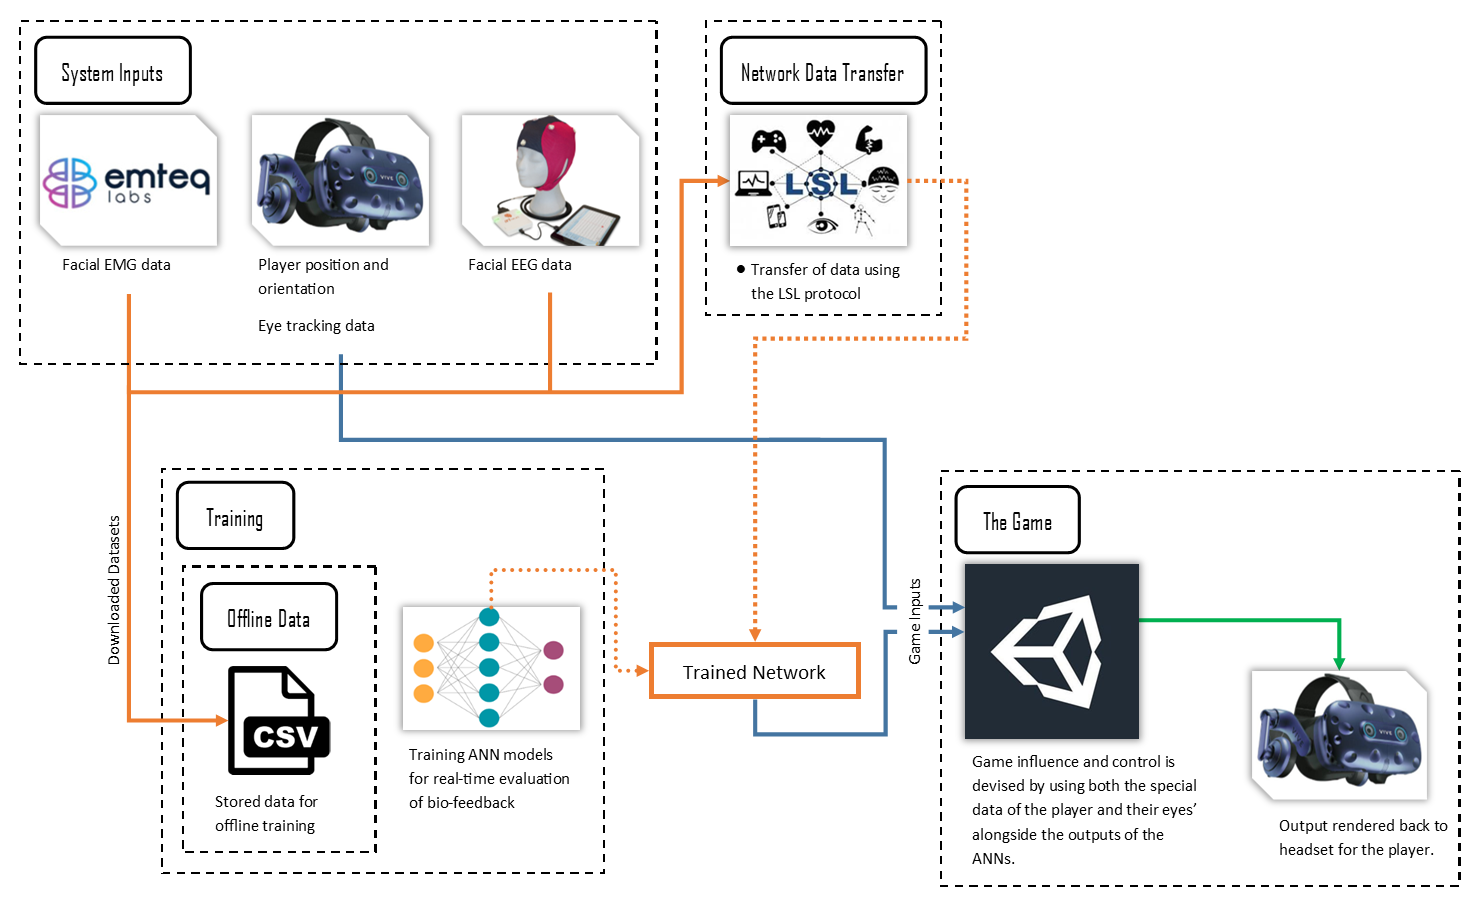
\includegraphics[width = 0.9 \linewidth] {[ Figures ]/System Diagram.png}
	\caption{System diagram: How input data from the specified technologies will be accessed and used within the game.}
	\label{fig:system_diagram_:_generic}
\end{figure}



The game was developed in the game engine Unity 3D. To use the data from the VR, EEG and EMG devices, each technology was integrated into the engine using C\#, and a variety of packages provided by and for Unity. The game itself consisted of a pair of two mini-games, both focusing on potential aspects of how a system like this could reasonably be used in a real world example. 


\begin{figure}[H]
	\centering
	\begin{subfigure}[t]{0.45\linewidth}
		
\includegraphics[width = \linewidth] {[ Figures ]/Get Figure.png}
		\caption{Concentration based difficulty, Breakout mini-game.}
		\label{fig:the_game_1}
	\end{subfigure}
	\begin{subfigure}[t]{0.45\linewidth}
		
\includegraphics[width = \linewidth] {[ Figures ]/Get Figure.png}
		\caption{Motor imagery controlled, sequence mini-game.}
		\label{fig:the_game_2}
	\end{subfigure}
	\caption{Screen shots of the game.}
	\label{fig:the_game}
\end{figure}


The first, \reffigure{fig:the_game_1}, was a clone of the arcade game Breakout \addcitation{}, in which the players aim is to break each block on the games board by bouncing a ball into them using a movable paddle, placed at the bottom of the play area. The intent with this part of the project was to allow the player to be able to effect the game world through an indirect influences, in this case, through the scaling of game difficulty. This was done by classifying the players state of relaxation and concentration, increasing and decreasing the balls movement speed based what state the neural networks within the system determines the focus level to be.

The second mini-game, \reffigure{fig:the_game_2}, was about repeating a randomised sequence of colours. The player would be tasked with repeating this sequence back, by activating crystals of the same colours in the same order. This mini-game was used to explore the concepts of motor-imagery based avatar control. This was accomplished by requiring the player to activate a crystals by lifting one of the avatars arms up. To accomplish this the player was required to think left-wards or right-wards and in doing so the avatar would begin lifting the chosen hand forwards. 






\pagebreak
%System Inputs
\subsection{System Inputs}	
Research into the different input methodologies demonstrated 


\begin{figure}[H]
	\centering
	
\includegraphics[width = 0.7 \linewidth] {[ Figures ]/Get Figure.png}
	\caption{System diagram: The input devices for the entire system.}
	\label{fig:system_diagram_:_inputs}
\end{figure}


\subsubsection{EEG}	
The recording of live EEG data is achieved through the sampling of voltage potentials across a subjects scalp. This is done through the use of a sensor array, the signals collected from these sensors are then collated within an amplifier, such as the EEGO Sport, and accessed in the form of a stream of float channels, usually one channel per sensors. Finally to record this data the amplifier is then connected back to a host computer, in which the saving and recording of the data is completed. The usages of this technology within the project will be specificity for motor imagery, and relaxation and concentration classification. Accessing this data live will be discussed in the networking part of this paper, however worth noting is that, due to the impractical nature of constant EEG tests, the large majority of this project was built around spoofing live EEG data using offline recordings. The specific ways in which this will be achieved will also be covered later in this paper.


\subsubsection{EMG}	
Similarly with EEG, EMG is the recording of the ambient voltage of the body, however specifically for EMG this comes from the activation of motor neurons. By placing these sensors across the certain regions of the body, the activity of muscular movements can be recorded and understood. The use of this technology within this project was focused around the eye, where it was used to detect when the player would blink. The purpose of this was to be able to detect and cease the effects of any EEG data on the game during the times a player blinked, this was seen as a requirement to the large amount of interference the movement of facial muscle can cause upon EEG recordings. In parallel to that of the EEG, pre-record sessions of normal and blinking EMG data was also used in the stead of requiring access to live data each time the project need to be tested. 



\subsubsection{VR}	
Though this system was initially intended for the use of the HTC Vive Pro Eye, with Unity's XR Interaction Tool-kit package the specific headset used within the project is a bit less consequential, due to the new input system adapting interactions to action bindings, rather then using the original method for managing game inputs using if statements. Using the this package, tracking data accessed from almost any headsets can be very easily bound as an action in the interaction asset. Headsets do however require that a project to be built for a specific platform, such as Android or Windows. With the intent of building this project for the HTC Vive however, the build platform can remain as Windows. In addition, this allowed for a mouse and keyboard solution to also be integrated into the project, to replace the inputs given via the headsets. This was important to do as it allowed for faster and less cumbersome testing of the solution. This replaced the headsets orientation tracking with a parametric based look function controlled via the mouses movement delta, as well as control over the paddle in breakout using the `A' and `D' keys, instead of inputs from the headsets controller.




\pagebreak
%Network Data Transfer
\subsection{Cross Network Data Transfer}	
Unlike accessing data from both the VR headset and the Emteq Pro, where both maintain a direct physical connection to the games host device, accessing EEG data is more complicated. As stated previously, sampling EEG data is done through connecting the sensors to an amplifier and then the amplifier to a separate computer for recording, however to maintain an undisturbed and interference free sample collection this system must be separate from that of the system the game is running on. This creates a new problem, how to access the data generated on a separate machine across a local network, and more specifically how to access this data in as close to real-time as possible.


\begin{figure}[H]
	\centering
	
\includegraphics[width = 0.7 \linewidth] {[ Figures ]/Get Figure.png}
	\caption{Data transfer across the local network using the LSL protocol.}
	\label{fig:networking_diagram}
\end{figure}


\subsubsection{LSL}	
For this to be done the solution of the LSL protocol \ccite{labstreaminglayer} was explored. LSL offers time-synchronous multi-type data transfer across local networks. Fortunately systems like the EEGO Sport come with software that supports this protocol by default, this has allowed for the distribution of all live data recorded from the head-wear to be accessed by any device on the network.

  
\subsubsection{Integration with Unity}	
However, though the broadcasting of EEG data via LSL, using software like EEGO, is inconsequential, accessing these streams within Unity requires a bit more work. To do this the 'liblsl-Csharp' package was used. This package allows for the integration of the LSL protocol into Unity through C\# scripting, requiring only the inclusion of the provided LSL.cs file, a C\# scripting file, and a specific .dll, library file, matching the games build platform. The library file used in the project is determined by the VR headset that a game is being built for, in the case that this projects aims to build on a device like the HTC Vive, the required library was LSL's Windows .dll. However for headsets like the Pico G2 4KS and the Oculus Quest, an Android based library will need to be built for the specific version of Android these headsets are running. 

\commentintext{Maybe talk about the actual C\# scripts in as an extra paragraph}
\commentintext{Also talk about the spoofing of the EEG and EMG data using LSL}




\pagebreak
%Machine Learning
\subsection{Machine Learning}	
Even with the data accessible within Unity, understand a meaning from the data is more complicated, and requires a more involved solution. Taking these inputs at face value, both the EEG and EMG data returns a series of float values each sample, in the form of either a list or array. Manually testing these numbers directly within Unity wasn't a viable solution, due to how individually these values are somewhat meaningless. Instead the projected opted for the use of pre-trained FFNNs (Feed Forward Neural Networks) within the game, this would allow for an analysis of the patterns forming within the data set as a whole. From this, three networks were developed for the project, each was tasked with the classification of both the EEG and EMG streams, into the given outputs: for the motor-imagery portion of the project the networks were trained to classify the likelihood between, an imagined left, right and neutral state; as for the concentration based network, EEG data was once again used to determine between a state of relaxation and of concentration; while lastly, the final network used EMG data to classify between the opening and closing of a players eyes.


\begin{figure}[H]
	\centering
	
\includegraphics[width = 0.7 \linewidth] {[ Figures ]/Get Figure.png}
	\caption{Artificial neural networks, there inputs and outputs.}
	\label{fig:system_diagram_:_machine_learning}
\end{figure}


\subsubsection{Keras}	 
To create these networks the Python library Keras \ccite{keras} was used. Keras is an interface library for Google Brains TensorFlow \cciteyear{tensorflow}, another python library used for the creation and training neural networks. Using the offline motor-imagery, relaxation and focus, and eye movement data sets mentioned in the System Inputs section of this paper, a model using `Binary Cross-Entropy' was generated for each. These models where originally designed with a hidden layer 20\% the size of the input layer, as shown in \reffigure{fig:ffnn_:_original_motor_imagery}. However the results of this network after several hours of training didn't appear promising

\begin{figure}[H]
	\centering
	\begin{subfigure}[t]{0.45\linewidth}
		
\includegraphics[width = \linewidth] {[ Figures ]/Get Figure.png}
		\caption{Example of the original FFNN used in the project.}
		\label{fig:ffnn_:_original_motor_imagery}
	\end{subfigure}
	\begin{subfigure}[t]{0.45\linewidth}
		
\includegraphics[width = \linewidth] {[ Figures ]/Get Figure.png}
		\caption{Example of the updated FFNN using more hidden layers, where the size of each is also larger.}
		\label{fig:ffnn_:_200_node_layer_motor_imagery}
	\end{subfigure}
	\caption{Manually designed networks.}
	\label{fig:ffnn_:_networks}
\end{figure}

Instead, the trialling of network architectures designed with more varied shapes and larger epoch counts began. Quickly, better accuracy's started to appear, the most promising of which where shown with networks that contained at least 2 or more hidden layers, and where the first layers node count exceeded 200.

This again was not much of a success, even with the higher accuracy, sitting at around 90\%, when compared against unseen (validation) data the accuracy became equal to that of random chance.


\subsubsection{Keras Tuner}
Due to the lack of accuracy given by the manually designed FFNN's: the unlikely chance that with the continued testing against human designed networks resulting in any reasonably accurate networks; and the slow speed in which fairly testing these networks required; it was clear that another solutions was again needed. This solution emerged as hyper-parameter optimisation, specifically the library Keras-Tuner \ccite{omalley2019kerastuner}. Keras-Tuner allows for the automation of neural networks by generating and training through the use searching algorithms. 
There are 3 types of tuner algorithms supported by Keras-Tuner, `Random Search', `Hyperband' and `Basyesian Optimisation'. Tests where performed over each of these tuners to test the creation of each of the three FFNN's needed for the project. After a while the choice was made to keep basyesian optimisation tuner for the networks as it showed the most success in predicting a high validation accuracy.

The inputs used for the network tuners are as shown in \reftable{tab:ffnn_:_search_parameters}. Having ran this for a while for each of the networks....

\commentintext{Talk about how the networks performed, ANN for motor imagery is rubbish, but the eye one is decent}

\begin{table}[H]
	\centering
	\begin{tabular}{ |c|c| }
		\hline
		
		Parameter 								& Value 							\\	\hline \hline
		
		Objective 								& `val\_accuracy' 					\\ 	\hline
		Layers 									& 1 to 6 							\\ 	\hline
		Nodes 									& 4 to 512, in steps of 4 			\\  \hline
		Hidden layer activation function 		& `relu', `sigmoid', `softmax' 		\\	\hline
		Output layer activation function 		& `relu', `sigmoid', `softmax' 		\\	\hline
		Learning rate 							& 0.01, 0.001, 0.0001 				\\	\hline
		Early stopping callback rate			& `val\_loss' 						\\  \hline
		Early stopping patience					& 3 								\\	
		
		\hline		
	\end{tabular}
	\caption{Input parameters used for tuning network search generation.}
	\label{tab:ffnn_:_search_parameters}
\end{table}



\subsubsection{Baracuda}	

\commentintext{How where the networks put into Unity}
\commentintext{What was my initial test case, the box moving?}





\pagebreak
%The Games
\subsection{The Implementation of the Game}


Though this project is designed to work on a VR headset with real-time EEG and EMG data provided, testing resulted in building the project for Windows PC's with the a mouse / keyboard input system, alongside running the offline EEG and EMG data to supply a valid prototyping environment without the need for the access to both equipment and participants.  

\commentintext{Player State Machine?}
\commentintext{Moving controls, per state?}
\commentintext{parametric look function?}
\commentintext{How the networks where used?}
\commentintext{Blocking of network inputs for blinking?}
\commentintext{Visual indecation of player ANN states, blink idecator and the focus bar?}
\commentintext{Lerping of everything?}
\commentintext{growth rate?}

\commentintext{Spawning of levels?}
\commentintext{level interaction code?}



















\pagebreak
\section{Conclusion and Future Work}

\subsection{Conclusion}
I conclude something...


\subsection{Future Work}			% - 300 Words
I want to do this in the future....


		% - 300 Words

\pagebreak
\printbibliography[notkeyword = software, title = References]

\pagebreak
\printbibliography[keyword = software, title = Software]

\end{document}
